%-------------------------------- Configurações --------------------------------

\documentclass[a4paper,         % Tamanho do papel: A4
	           abntfigtabnum,
	           noindentfirst,
	           normaltoc,
	           pnumplain,
	           notimes
	           % capchap,
]{abnt}

% Links border color
\newcommand{\bc}{NavyBlue}

\usepackage[utf8]{inputenc} % para pode escrever caracteres acentuados normalmente
\usepackage[brazil]{babel}
\usepackage{graphicx}
\usepackage[usenames,dvipsnames]{xcolor} % http://en.wikibooks.org/wiki/LaTeX/Colors
\usepackage[pdfborder={0 0 0},pdfborderstyle={/S/U/W 0.5},citebordercolor=\bc,filebordercolor=\bc,urlbordercolor=\bc,linkbordercolor=\bc]{hyperref} % http://www.tug.org/applications/hyperref/manual.html e http://migre.me/7FH3e
\usepackage[alf]{abntcite}
\usepackage{booktabs} % para utilização das linhas separadoras na tabela
\usepackage{listings} % http://linorg.usp.br/CTAN/macros/latex/contrib/listings/listings.pdf
\usepackage{textcomp}
\usepackage{minted} % foi adicionado o seguinte hack no minted: http://migre.me/7M8wI

%--------------------------- Minted Highligthing -------------------------------

\renewcommand\listingscaption{Código}

% http://github.com/hugomaiavieira/pygments-style-github
\usemintedstyle{github}

% O minted é tipo uma extensão do fancyvrb. Então, algumas modificações nele
% são feitas de acordo com o fancyvrb.
% Documentação do fancyvrb: http://linorg.usp.br/CTAN/macros/latex/contrib/fancyvrb/fancyvrb.pdf

% Ajustar o estilo do número, de acordo com o fancyvrb.
\renewcommand{\theFancyVerbLine}{\textcolor{Gray}{\scriptsize\arabic{FancyVerbLine}}}

% Ajusta estilo do caption. http://linorg.usp.br/CTAN/macros/latex/contrib/caption/caption-eng.pdf
\usepackage{caption}
\DeclareCaptionStyle{code_style}{margin=2mm}
\DeclareCaptionFont{code_font}{\footnotesize\bfseries}
\captionsetup[listing]{style=code_style,labelfont=code_font,textfont=code_font}

% Criando um novo comando para facilitar a adição de códigos
% http://tex.stackexchange.com/questions/42393/new-environment-with-minted
\makeatletter
\newenvironment{mycode}[3]
 {\VerbatimEnvironment
  \minted@resetoptions
  \setkeys{minted@opt}{linenos,fontfamily=courier, fontsize=\scriptsize, xleftmargin=21pt}
  \renewcommand{\minted@proglang}[1]{#1}
  \begin{listing}[h]
    \caption{#2}\label{#3}
      \begin{VerbatimOut}{\jobname.pyg}}
 {\end{VerbatimOut}
  \minted@pygmentize{\minted@proglang{}}
  \DeleteFile{\jobname.pyg}
  \end{listing}}
\makeatother

%--------------------------------- Informações ---------------------------------

% http://www.tug.org/applications/hyperref/manual.html
\hypersetup{
  pdftitle=Técnicas emergentes de desenvolvimento de software,
  pdfauthor=Hugo Henriques Maia Vieira
  % pdfsubject={},
}

\begin{document}

\titulo{Técnicas emergentes de desenvolvimento de software}
\autor{Hugo Henriques Maia Vieira}
\instituicao{Universidade Estadual do Norte Fluminense Darcy Ribeiro}
\orientador[Tutor: ]{Rodrigo Soares Manhães, M.Sc.}
\comentario{Monografia apresentada ao Curso de Graduação em Ciência da
Computação da Universidade Estadual do Norte Fluminense Darcy Ribeiro como
requisito para obtenção do título de Bacharel em Ciência da Computação, sob
orientação do Prof. Rodrigo Soares Manhães, M.Sc.}
\local{Campos dos Goytacazes/RJ}
\data{2011}


\capa
\folhaderosto

\include{epigrafe}
\begin{center}
\textbf{AGRADECIMENTOS} \\ [2.5cm]
\end{center}

À meu pai Roosevelt, meu melhor amigo e grade companheiro, por estar sempre presente em todos os momentos felizes e tristes da minha vida e por ser a pessoa mais importante da formação do meu caráter, por eu me tornar quem sou.

À minha mãe e minhas irmãs, que mesmo distantes estão sempre por perto.

À minha namorada Alice, pelo amor, companheirismo e paciência.

Ao amigo e professor Rodrigo, por me mostrar o caminho da luz e por ser meu grande mestre e orientador.

À professora Sahudy, por ter sido parte fundamental da minha formação, acadêmica, profissional e pessoal.

À professora Annabell, por todo companheirismo e carinho, por mostrar que o trabalho duro é recompensador.

Ao professor Rivera por sua dedicação ao buscar sempre um curso melhor.

Ao professor Rogério, representando o NSI, por ter me aberto as portas para a área que adoro e escolhi seguir em minha vida profissional.

À todos meu amigos de curso, especialmente meus também companheiros de Algorich, Eduardo, Herond e Rafael por estarem presentes nos momentos mais dramáticos e nos mais engraçados.

À toda minha família, meus avós, meus primos e meus tios, por todo o suporte e felicidade que me proporcionam sempre.

\listoffigures

\begin{resumo}
Aqui entra o resumo do meu trabalho que será a última coisa a ser feita.
\end{resumo}

\sumario

\chapter{Introdução}

A tecnologia e os negócios mudam e evoluem de modo extremamente rápido hoje e o mercado demanda e espera software inovadores e de alta qualidade, que sejam adequados a suas necessidades e desenvolvidos o mais rápido possível \cite{TheBusinessOfInnovation}.

O desenvolvimento ágil de software, que neste ano de 2012 completa 11 anos, foi elaborado visando atender estas expectativas do mercado \cite{AgileManifesto}, focando o processo de desenvolvimento nas pessoas e abraçando as mudanças que naturalmente surgem durante o desenvolvimento do software.

Como a adoção do desenvolvimento ágil é crescente nos últimos anos \cite{ResumoChaosReport}, diversos métodos e técnicas vem sendo desenvolvidos, tendo como base os princípios e valores ágeis \cite{BDDRodrigo}, principalmente relacionadas ao teste de software. Contudo, estes métodos e técnicas continuam em evolução, tendo alguns de seus pontos ainda em aberto.

Este trabalho pretende contextualizar e discutir a utilização de técnicas emergentes de teste de software, aqui definidas como Desenvolvimento Guiado por Testes (do inglês, \textit{Test-Driven Development} - TDD)\nomenclature{TDD}{Test-Driven Development}, Desenvolvimento Guiado por Comportamento (do inglês, \textit{Behaviour-Driven Development - BDD})\nomenclature{BDD}{Behaviour-Driven Development}, Integração Contínua e Dublês de Teste. Para esta contextualização, será utilizado um sistema web desenvolvido pelo autor aplicando tais técnicas: o kanban-roots.

\section{Justificativas e objetivos}

São encontrados alguns poucos trabalhos relacionados ao tema abordado nesta monografia, como constata \citeonline{BDDSolis}. Sendo assim, o objetivo do presente trabalho é oferecer um estudo teórico-prático das técnicas emergentes na área de teste de software com metodologias ágeis de desenvolvimento, visando de agregar conhecimentos ora dispersos e difusos, sobre as diferentes abordagens, possibilidades e pontos em aberto no emprego de tais técnicas.

As técnicas que serão abordadas neste trabalho tiveram seu conceito definido no mercado e evoluem através da evolução das ferramentas que as implementam. Na figura \ref{img:fluxo_conceito_ferramenta} pode-se visualizar o fluxo de evolução onde primeiramente cria-se um conceito e, em seguida, uma ferramenta que o implemente. Com base na utilização e observação desta ferramenta, há uma percepção de novas necessidades, fazendo que os conceitos evoluam e novas ferramentas sejam criadas.

\begin{figure}[h]
  \center
  \caption{Fluxo de evolução dos conceitos e ferramentas}
  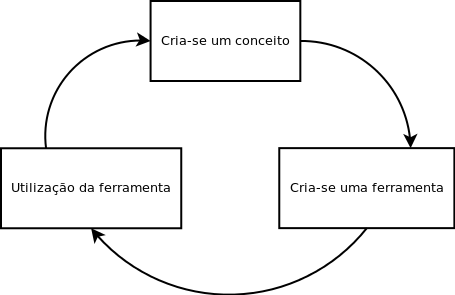
\includegraphics[scale=0.60]{images/fluxo-conceito-ferramenta}
  \label{img:fluxo_conceito_ferramenta}
\end{figure}

Desta forma, a evolução das ferramentas e a evolução conceitual estão intimamente ligadas. No texto original sobre BDD \cite{IntroducingBDD} já se encontra isto. A inspiração para a criação de BDD foi uma ferramenta chamada \textit{AgileDox}\footnote{Mais informações em \url{http://agiledox.sourceforge.net}}, que fez o autor da mesma antever as novas possibilidades que então cristalizou no conceito de BDD. Justamente por esta característica dinâmica de evolução, as informações e os diferentes conceitos sobre as técnicas estão dispersos, pois nunca foram sistematizados, ficando em uma espécie de ``inteligência coletiva"\ da comunidade de desenvolvimento ágil.

Além disso, como o presente trabalho está no contexto dos métodos ágeis, e nestes as partes conceitual e prática formam um todo inseparável, para toda técnica abordada serão exemplificados os conceitos usando o código de uma ferramenta web, denominada kanban-roots, desenvolvida pelo próprio autor do presente trabalho, utilizando práticas ágeis de desenvolvimento, especificamente Desenvolvimento guiado por Testes (TDD) e Desenvolvimento guiado por Comportamento (BDD).

\section{Metodologia}

Para atingirmos os objetivos propostos neste trabalho, será feita uma explanação sobre cada uma das técnicas emergentes estudadas, aqui definidas como:

\begin{itemize}
  \item Desenvolvimento guiado por testes (TDD, do inglês \textit{Test-Driven Development})
  \item Desenvolvimento guiado por comportamento (BDD, do inglês \textit{Behaviour-Driven Development}
  \item Integração contínua
  \item Dublês de teste
\end{itemize}

Serão comparadas as diferentes abordagens, possibilidades, pontos em aberto no emprego de cada técnica, observando a aplicabilidade de cada uma delas e a eficiência respectiva.

Como base para a discussão, será utilizado o kanban-roots\footnote{\url{http://github.com/hugomaiavieira/kanban-roots}}, que será apresentado na Seção \ref{sec:kanban_roots}. O kanban-roots é um projeto que foi desenvolvido pelo autor do presente trabalho utilizando todas as técnicas abordadas neste, possibilitando desta forma a obtenção de dados e experiências da utilização das técnicas em um projeto real.

Todos os trechos de código apresentados neste trabalho são trechos retirados do kanban-roots e a primeira linha de cada trecho sempre será um comentário informando o nome do arquivo original em que o referido trecho se encontra.

\section{Ferramentas utilizadas}

Para o desenvolvimento do kanban-roots foram utilizadas diversas ferramentas, sendo importante citar em que contexto e momento cada uma delas é utilizada.

Como base para o desenvolvimento, foi utilizado o \textit{framework web} Ruby On Rails\footnote{\url{http://rubyonrails.org}} que é escrito utilizando a linguagem de programação Ruby. Para os testes de unidade apresentados na Seção \ref{sub:tdd} foi utilizado o Test::Unit\footnote{\url{http://test-unit.rubyforge.org/}}. Já na Seção \ref{sub:bdd} é utilizado o Rspec\footnote{\url{http://rspec.info/}} para testes unitários, testes de aceitação e dublês de teste. Ainda na Seção \ref{sub:bdd} também foi utilizado o Cucumber\footnote{\url{http://cukes.info/}} para testes de aceitação. Além dessas ferramentas, também foi utilizado o FactoryGirl\footnote{\url{https://github.com/thoughtbot/factory_girl}} para \textit{fixtures replacement} em todos os momentos em que se fez necessário. Foram ainda utilizados os banco de dados SQLite\footnote{\url{http://www.sqlite.org/}}, em ambiente de desenvolvimento, e o MySQL\footnote{\url{http://www.mysql.com}}, em ambiente de produção.

\section{Organização}
\label{sec:organizacao}

No Capítulo 2 será fundamentado os diferentes tipos de teste de software bem como as técnicas emergentes abordadas no presente trabalho. No Capítulo 3 serão contextualizadas as técnicas emergentes de teste de software, discutindo suas abordagens e pontos em aberto. No Capítulo 4 são apresentadas as conclusões obtidas e os trabalhos futuros.
\chapter{Fundamentação teórica}

\section{Desenvolvimento de software}
\label{sec:desenvolvimento_de_software}

O desenvolvimento de software é o ato de elaborar e implementar um sistema computacional que transforme as necessidades de um utilizador ou de um mercado em um produto de software.

O desenvolvimento de software é essencialmente uma atividade intelectual e criativa, exigindo a manipulação de uma gama muito grande de conhecimentos e informações. Além disso, os desenvolvedores de um software se preocuparem com o conteúdo e estrutura, além de deverem se preocupar também com o comportamento fazendo com o que o desenvolvimento de software seja uma atividade complexa, devendo ser realizada por especialistas munidos de técnicas que os auxiliem da melhor maneira possível.


\subsection{Agilismo}
\label{sub:agilismo}

Em 2001 um grupo de dezessete especialistas, reconhecidos pela comunidade como grandes nomes do desenvolvimento software, se reuniram para discutir sobre um crescente conjunto de métodos que vinham surgindo e decidiram usar o termo Agilismo para descrever essa nova geração de métodos \cite{AgileStory}. Na mesma reunião, eles também escreveram o Manifesto Ágil \cite{AgileManifesto}, delineando um conjunto de valores e princípios que, em resumo, trilham um caminho para a eliminação de documentação e processos desnecessários, buscando a simplicidade, com foco na geração de valor e proximidade com o cliente, além de possibilitar respostas rápidas e eficazes às mudanças. Desde então, os métodos ágeis vêm ganhando projeção e importância no cenário da produção de software.

Pode-se dizer então, que o Desenvolvimento Ágil, ou Agilismo, é um rótulo genérico para os métodos de desenvolvimento de software baseados no Manifesto Ágil.

É importante citar que o desenvolvimento ágil sofreu grande influência de um conceito conhecido como \textit{Lean Thinking} (``pensamento enxuto"\ em português), uma linha de pensamento em gestão baseada nos princípios de \textit{Lean Manufacturing}\footnote{Os princípios de \textit{Lean Manufacturing} são originários do sistema Toyota de produção, que propôs um modo inteiramente novo de pensar a respeito de fabricação e logística de automóveis.} que se caracteriza por produção em pequenos lotes, eliminação de desperdícios, obsessão com qualidade, equipes multifuncionais praticando aprendizado contínuo, melhoria contínua de processo, sistema puxado de produção e a qualidade sendo responsabilidade dos trabalhadores como um todo \cite{BDDRodrigo}.

Uma das premissas do agilismo é que os custos de alterações sejam praticamente linear ao longo do tempo, independente do ponto em que esteja, fazendo com que a curva de custo de alterações seja semelhante à apresentada na Figura \ref{img:custo-agile}.

\begin{figure}[h]
  \center
  \caption{O custo das modificações no modelo ágil - Fonte: \cite{XPKent}}
  \includegraphics[scale=0.45]{images/custo-agile}
  \label{img:custo-agile}
\end{figure}

Isto é conseguido porque nos métodos ágeis não é feito um planejamento inicial muito abrangente. Ao invés disso, o desenvolvimento é dividido em iterações curtas (de uma a quatro semanas), onde ao início de cada uma delas é feito um novo planejamento, corrigindo o curso do projeto com base no \textit{feedback} obtido nas iterações anteriores. Para isso, a proximidade e interação do cliente com o projeto deve ser constante. Desta forma, o desenvolvimento é baseado em \textit{feedback} concreto e não em especulações sobre o futuro, fazendo com que o aprendizado permanente leve a melhorias e torne o produto final mais adequado para o seu público, além de o tornar mais simples e sem elementos extras que poderiam ser utilizados no futuro. Além disso, os testes automatizados são fundamentais para que as modificações realizadas não alterem o comportamento atual do sistema  \cite{XPKent}, dando segurança para que estas sejam feitas, além de permitir que o código melhore continuamente.

Ao utilizar métodos ágeis como \textit{eXtreme Programming} (XP) \nomenclature{XP}{eXtreme Programming} e Scrum, todas as funcionalidades do sistema são levantadas através de histórias, que são escritas pelo próprio cliente em pequenos cartões. A equipe de desenvolvimento utiliza os cartões para saber quais funcionalidades são desejadas pelo cliente. Contudo, os cartões podem acabar representando histórias que consomem muito esforço para serem implementadas. Nesse caso, a equipe divide os cartões em tarefas, que são registradas em novos cartões para serem distribuídas facilmente entre os desenvolvedores. Na Figura \ref{img:projeto_agile} é mostrada divisão de um projeto nos métodos ágeis.

\begin{figure}[h]
  \center
  \caption{Divisão de um projeto nos métodos ágeis}
  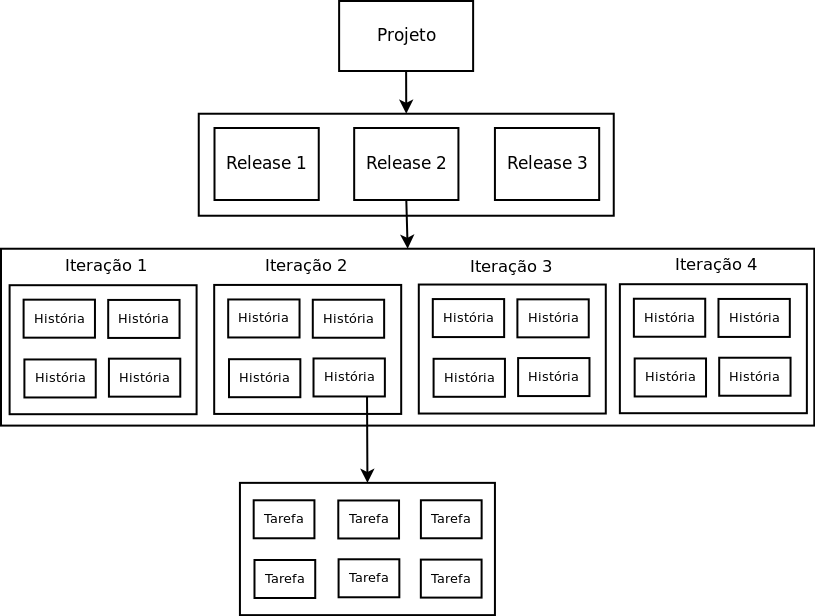
\includegraphics[scale=0.45]{images/projeto}
  \label{img:projeto_agile}
\end{figure}

No início do projeto o cliente e a equipe de desenvolvimento dividem o projeto em \textit{releases}, que são entregas de software que implementem um conjunto de funcionalidades que possui um valor bem definido para o cliente. Essas entregas são feitas de forma incremental, e em um espaço de tempo não muito longo (geralmente dois meses), para que o cliente possa começar a utilizar e obter os benefícios que elas oferecem, além de dar o \textit{feedback} necessário para que sejam feitas melhorias. Depois de definida a primeira \textit{release}, o cliente escreve as histórias que serão implementas nesta. As histórias das \textit{releases} posteriores podem ser deixadas para o futuro, pois durante o desenvolvimento de cada \textit{release} o cliente irá utilizar o software diversas vezes, o que irá influenciar as histórias das próximas \textit{release}. Durante a \textit{release} o cliente pode alterar as histórias se considerar necessário, podendo assim incorporar o aprendizado adquirido com o uso do sistema.

Uma \textit{release}, mesmo que seja pequena, representa um tempo ainda grande, pois não se deve esperar tanto tempo para ter o \textit{feedback} da utilização do software pelo cliente. Assim, ela é dividida em um conjunto de iterações, que são basicamente um pequeno espaço de tempo (geralmente duas semanas) dedicado para a implementação de um conjunto de histórias. A diferença entre uma \textit{release} e uma iteração é que na iteração o cliente não pode alterar as histórias definidas, pois a mudanças muito frequentes ao longo do trabalho da equipe de desenvolvimento prejudicam o ritmo de programação, pois confundem os desenvolvedores. No início de cara iteração é feita uma reunião para o planejamento da mesma, de modo que cliente e equipe de desenvolvimento definam as histórias que serão implementadas na iteração. Ao final de cada iteração e cada \textit{release}, o cliente tem novas histórias implementadas, ou seja, software funcionando. Dessa forma, ele poderá utilizar o sistema com as novas funcionalidades, tornando o \textit{feedback} ainda mais efetivo.

Mas para que isso seja possível, os métodos ágeis contam com um conjunto de técnicas para dar suporte a seu caráter iterativo e incremental, sendo algumas destas técnicas abordadas mais adiante neste trabalho.


\section{Teste de software}
\label{sec:teste_de_software}

A maneira como o teste de software é aplicado varia de acordo com a metodologia utilizada no desenvolvimento. Tradicionalmente o teste de software é feito somente após o desenvolvimento ter sido concluído \cite{TesteSoftware, Pressman}. Já nos métodos ágeis um sentido oposto é seguido \cite{ArtOfAgileDevelopment}, sendo utilizadas técnicas como \textit{Test-Driven Development} (abordada na Seção \ref{sub:tdd}) e \textit{Behaviour-Driven Development} (abordada na Seção \ref{sub:bdd}).

O uso de estratégias nas quais a escrita dos testes automatizados é feita antes do código de implementação das funcionalidades, como TDD e BDD, não exclui o emprego de técnicas de teste de software tradicionais como classes de equivalência, análise do valor limite, análise da complexidade ciclomática e outras.

Os próximos tópicos definirão os tipos de teste utilizados no contexto do presente trabalho.


\subsection{Testes de unidade}
\label{sub:testes_de_unidade}

Testes de unidade são testes nos quais unidades individuais do sistema são testadas para determinar se estão aptas para uso. Uma unidade é a menor parte testável de uma aplicação. Em programação procedural uma unidade pode ser uma função. Já em programação orientada a objetos, uma unidade pode ser um método ou uma responsabilidade da classe. \citeonline{TesteSoftware} afirmam que neste contexto, espera-se que sejam identificados erros relacionados a algoritmos incorretos ou mal implementados, estruturas de dados incorretas, ou simplesmente erros de programação.

Para exemplificar, no Código \ref{code:unit_test_spec} é apresentado o teste de unidade para o método \texttt{Category\#name\_as\_css\_class}, cuja implementação é mostrada no Código \ref{code:unit_test}. Este método transforma o nome da Categoria em um nome de classe CSS\footnote{\textit{Cascading Style Sheets}. Mais em \url{http://pt.wikipedia.org/wiki/Cascading_Style_Sheets}}\nomenclature{CSS}{Cascading Style Sheets}, deixando todos seus caracteres em minúsculo e substituindo os caracteres / (barra),  (espaço) e - (traço) por \_ (sublinhado).

\begin{mycode}{rspec}%
{Teste de unidade automatizado para o método \texttt{Category\#name\_as\_css\_class} }{code:unit_test_spec}
# spec/models/category_spec.rb
describe Category do
  it "should return its name as a css class" do
    category = Factory.build :category, :name => "Feature"
    category.name_as_css_class.should == "feature"

    category.name = "New Feature"
    category.name_as_css_class.should == "new_feature"

    category.name = "Other-New Feature"
    category.name_as_css_class.should == "other_new_feature"

    category.name = "Study/Research"
    category.name_as_css_class.should == "study_research"
  end
end
\end{mycode}

\begin{mycode}{rspec}%
{Implementação do método \texttt{Category\#name\_as\_css\_class} }{code:unit_test}
# app/models/category.rb
class Category < ActiveRecord::Base
  def name_as_css_class
    self.name.downcase.gsub(/\/| |-/, "_")
  end
end
\end{mycode}


\subsection{Testes de integração}
\label{sub:testes_de_integracao}

No contexto do presente trabalho, os testes de integração testam as integrações do código com o mundo exterior. Eles podem ser testes que se comuniquem através da rede, tenham contato com o sistema de arquivos ou deixem os limites de seu próprio processo \cite{ArtOfAgileDevelopment}.

Para exemplificar, será utilizada uma extensão criada para fazer o destaque da sintaxe de código na descrição das Tarefas e no conteúdo do Comentários no kanban-roots, como apresentado na Figura \ref{img:highlighting}. Para isso, é utilizado um \textit{framework} em Python chamado Pygments\footnote{ Mais em \url{http://pygments.org/}}.

\begin{figure}[h]
  \center
  \caption{Comentário com destaque da sintaxe de código no kanban-roots}
  \includegraphics[scale=0.5]{images/highlighting}
  \label{img:highlighting}
\end{figure}

O Pygments deve ser instalado na máquina onde o kanban-roots está sendo executado. No entanto, o kanban-roots foi projetado rodar em um servidor próprio ou em um VPS\footnote{ \textit{Virtual Private Server}. É um servidor em ambiente compartilhado que possui acesso \textit{root} e processos independentes para cada conta VPS criada.}, mas também no Heroku\footnote{ É um PaaS (\textit{platafom as a service}) que tem uma cota de utilização gratuita. No Heroku não é possível instalar dependências no sistema. Mais em \url{http://heroku.com}}. Sendo assim, foi utilizado um serviço gratuito e não oficial criado por Trevor Turk e hospedado no Google App Engine que permite a utilização da API \nomenclature{API}{Application programming interface} do Pygments através de um POST para o serviço. Dessa forma, deve-se testar a integração com o serviço e também a integração com o Pygments instalado localmente.

No Código \ref{code:integration_spec} é apresentado o teste de integração para o \textit{highlighting} de código englobando os dois casos citados anteriormente e no Código \ref{code:integration} é apresentada a implementação para esta fucnionalidade.

É importante perceber que, para isolar o teste, foi utilizado um dublê de teste (neste caso um \textit{stub}) para simular a resposta do método \texttt{can\_pygmentize?} que faz uma verificação no sistema operacional para identificar se o Pygments está instalado ou não. Dublês de teste serão abordados mais detalhadamente na Seção \ref{sub:dubles_de_teste}.

\begin{mycode}{rspec}%
{Teste de integração automatizado para o \textit{highlighting} de código}{code:integration_spec}
# spec/lib/albino_render_spec.rb
describe HTMLwithAlbino do
  before(:all) do
    @render = HTMLwithAlbino.new
    @code_text = 'puts "hello!"'
    @highlighted_code =
      "<div class=\"highlight\"><pre>" +
        "<span class=\"nb\">puts</span> <span class=\"s2\">&quot;hello!&quot;</span>\n" +
      "</pre>\n</div>\n"
  end

  it "should get the highlighted block code from pygments.appspot.com" do
    @render.stub(:can_pygmentize?).and_return(false)
    @render.block_code(@code_text, "ruby").should == @highlighted_code
  end

  it "should get the highlighted block code from local pygments" do
    @render.stub(:can_pygmentize?).and_return(true)
    @render.block_code(@code_text, "ruby").should == @highlighted_code
  end
end
\end{mycode}

\begin{mycode}{ruby}%
{Implementação do \textit{highlighting} de código}{code:integration}
# lib/albino_render.rb
class HTMLwithAlbino < Redcarpet::Render::HTML
  def block_code(code, lang)
    if can_pygmentize?
      Albino.colorize(code, lang)
    else
      # This is a hack for pygments work on Heroku
      require "net/http"
      Net::HTTP.post_form(URI.parse("http://pygments.appspot.com/"),
                          {"code"=>code, "lang"=>lang}).body
    end
  end

  private
  def can_pygmentize?
    system "pygmentize -V"
  end
end
\end{mycode}


\subsection{Testes de aceitação}
\label{ssub:testes_de_aceitacao}

Testes de aceitação são especificações para o comportamento das funcionalidades de um sistema. Eles mostram se o sistema se comporta corretamente pela perspectiva de um usuário, sem nos dizer nada sobre como o sistema implementa esse comportamento \cite{TestDrivenKoskela}. Além disso, é verificada a integração entre as diversas unidades que interagem para prover esta funcionalidade.

Relacionando com os métodos tradicionais, os testes de aceitação implementam os casos de uso levantados na análise orientada a objetos.

No Código \ref{code:acceptance} são apresentados exemplos de teste de aceitação, utilizando BDD com a escrita em texto plano. O primeiro cenário testa a funcionalidade de clicar e arrartar as tarefas de uma posição para outra no kanban. Já o segundo cenário testa a funcionalidade de limpar a divisão \textit{Done} do kanban, ou seja, retirar do quadro todas as tarefas concluídas.

BDD e testes de aceitação serão vistos com mais detalhes na Seção \ref{sub:bdd}.

\begin{mycode}{cucumber}%
{Teste de aceitação para o registro de um contribuidor}{code:acceptance}
# features/board.feature
Feature: Use the board
  As a user
  I want use the board
  In order see, move and manipulate the taks of my project

  @javascript
  Scenario: Drag and drop a task to another board position
    Given I am an authenticated contributor
    And I have a project
    And the following tasks:
      | title  | position |
      | task 1 | Doing    |
      | task 2 | Done     |
    And I am on the projects board page
    When I drag "task 1" task to "Done" position
    Then I should see "task 1" task at "Done" position

  Scenario: Clean up Done tasks
    Given I am an authenticated contributor
    And I have a project
    And the following tasks:
      | title  | position |
      | task 1 | Doing    |
      | task 2 | Done     |
      | task 3 | Done     |
      | task 4 | Done     |
    When I am on the projects board page
    And I follow "Clean up Done"
    Then I should see "Done division was cleaned up."
    And the Done division should be cleaned
\end{mycode}


\section{Técnicas emergentes de teste de software}
\label{sec:tecnicas_emergentes_de_teste_de_software}

Nesta seção serão apresentadas, conceitualmente, as técnicas emergentes de teste de software, sendo elas o Desenvolvimento Guiado por Testes (do inglês, \textit{Test-Driven Development} - TDD), Desenvolvimento Guiado por Comportamento (do inglês, \textit{Behaviour-Driven Development - BDD}), Integração Contínua e Dublês de Teste.

\subsection{Test-Driven Development (TDD)}
\label{sub:tdd}

O \textit{Test-Driven Development} (Desenvolvimento guiado por testes) é uma técnica onde o desenvolvimento do software é guiado por \textbf{testes automatizados}, que são escritos antes de qualquer linha de código relativo a funcionalidades. Primeiro escreve-se um teste, depois escreve-se o código para passar neste teste. Em seguida, o código é refatorado para encontrar um design melhor, contando sempre com os testes existentes para que não sejam introduzidas falhas em outras partes do sistema.

Esta abordagem encoraja bom design \cite{GrowingOOByTests}, produz código testável e mantém longe a sobre-engenharia por conta de falsas suposições, pois, nos testes, é especificado o que é desejado e escreve-se o código para fazer apenas aquilo que realmente é necessário. \cite{TestDrivenKoskela, TDDbyExample, EmpiricalTDD}

\citeonline{EmergentDesign} relaciona o entendimento do problema e o fluxo natural do TDD:

\begin{citacao}
Tentar escrever um teste é uma boa maneira de testar a si mesmo sobre seu conhecimento sobre como a classe deverá funcionar antes de você escrevê-la. Esta é uma boa sequência: tenha certeza de que você entende o que você irá tentar fazer antes de você realmente tentar fazer. De fato, colocando dessa maneira, parece muito mais natural considerar os testes como Primeira Tarefa e criar o código como Segunda Tarefa. (tradução do autor)
\end{citacao}

O TDD vem sendo utilizado esporadicamente há anos, contudo, não existia um nome para identificar essa forma de desenvolver software, que no fim dos anos noventa, ganhou além do nome, uma definição. Atualmente, TDD começa a ganhar força e ser utilizada em times de grandes empresas como Google, Yahoo, Microsoft e IBM \cite{EmpiricalTDD}. O Anexo \ref{cha:a_efetividade_do_tdd} apresenta uma análise de diversos estudos sobre a efetividade de TDD na indústria e na academia.

\subsubsection{Ciclo TDD}
\label{ssub:ciclo_tdd}

Com base no trabalho de \citeonline{TDDbyExample}, o ciclo de desenvolvimento TDD é composto pelas seguintes etapas:

\begin{enumerate}
\item \textbf{Adicionar um teste}

Cada ciclo se inicia com a criação de um teste de unidade. Este teste inevitavelmente irá falhar, pois é escrito antes do código ser implementado de fato. Para escrever um teste, o desenvolvedor precisa entender claramente as especificações e requisitos da unidade. Isso faz com que o desenvolvedor tenha como foco os requisitos antes do código, o direcionando a escrever código apenas para o que é realmente necessário.

Além disso, segundo \citeonline{XPTeles}, ao se pensar e escrever o teste, está sendo feita também a análise e \textit{design} das classes do sistema.

\item \textbf{Executar todos os testes e ver se algum falha}

Todos os testes devem ser executados e o novo teste deve falhar pela razão esperada: a funcionalidade não foi desenvolvida. Isto aumenta a confiança que se está testando a coisa certa.

\item \textbf{Escrever código}

O próximo passo é escrever código \textbf{somente para que o teste passe}. O código poderá não ser perfeito, pois posteriormente ele será melhorado. O importante é que o código faça o mínimo para passar no teste. Segundo \citeonline{BDDRodrigo}:

\begin{citacao}
Enquanto código útil é um patrimônio que gera valor, qualquer código criado inutilmente é tempo desperdiçado e, no fim das contas, um fardo, que sem gerar valor algum, aumentará a complexidade geral do software.
\end{citacao}

\item \textbf{Executar os testes e ter sucesso}

Ao Executar os testes e todos eles passarem, o código possuirá todos os requisitos testados e o programador pode ficar confiante para melhorá-lo.

\item \textbf{Refatorar}

Esta é uma etapa muito importante, onde o código escrito anteriormente é melhorado. Segundo \citeonline{FowlerRefatoracao}, refatorar é reestruturar o software aplicando uma série de alterações em sua estrutura interna para torná-lo mais fácil de ser entendido e menos custoso de ser modificado, sem alterar seu comportamento observável.

Refatorar melhora o projeto do software, o torna mais fácil de entender e modificar, ajuda a encontrar falhas e ajuda o desenvolvedor a programar mais rapidamente.

Como na refatoração o comportamento do código não deve ser alterado, após refatorar e executar novamente os testes, todos eles devem passar.

\end{enumerate}

A figura \ref{img:ciclo-tdd} resume o ciclo TDD, onde as etapas 1 e 2 são representadas pelo item \textbf{teste}, as etapas 3 e 4 pelo item \textbf{codifique} e a etapa 5 pelo item \textbf{refatore}.

\begin{figure}[h]
  \center
  \caption{O ciclo TDD}
  \includegraphics[scale=0.45]{images/ciclo-tdd}
  \label{img:ciclo-tdd}
\end{figure}


\subsubsection{Design emergente}
\label{ssub:design_emergente}

\textbf{TODO: juntar isso com o mesmo tópico em contextualização?}

No contexto em que TDD costuma ser aplicado $-$ em processos ágeis, com um ciclo de vida iterativo-incremental $-$ não é realizado um amplo \textit{design} prévio. Sendo assim, o \textit{design} evolui incrementalmente, ou seja, o \textit{design} emerge de acordo com a necessidade. Sabendo disso, uma característica extremamente importante do TDD é a facilitação ao \textit{design} emergente, que muitos consideram ser sua a principal característica \cite{EmergentDesign}.

TDD é considerada uma técnica essencial para o \textit{design} emergente porque
quando se está escrevendo um teste anteriormente ao código, o programador contempla e decide não apenas a interface do software (i.e. nomes de classes/métodos, parâmetros, tipos de retorno, lançamento de exceções), mas também o comportamento do software (i.e. resultados esperados para determinadas entradas) \cite{JanzenTDD}.

Além disso, \citeonline{EmergentDesign} constata que o ponto de vista do teste pode passar informações sobre o design, porque o teste de uma classe funciona como o primeiro cliente da classe. Com isso, a interface que o teste sugere é uma interface dirigida ao cliente, sendo assim, geralmente é mais estável.

\citeonline{DammTDD} também afirmam que o TDD faz com que as pessoas pensem mais no design em vez de codificar precipitadamente sem saber o que implementar ainda e \citeonline{XPTeles} ressalta a importância da refatoração para a evolução incremental do design:

\begin{citacao}
Ao longo das iterações, o design precisa evoluir, mas deve manter-se simples e claro para que a equipe possa fazer alterações no software a qualquer momento, com facilidade. Por esta razão o \textit{refactoring} tem um papel fundamental no design.
\end{citacao}


\subsection{Behaviour-Driven Development (BDD)}
\label{sub:bdd}

Criado em 2006 \cite{IntroducingBDD}, \textit{Behaviour-Driven Development} (Desenvolvimento guiado por comportamento) é uma técnica de desenvolvimento de software cuja amplitude se estende às atividades de design, documentação, validação e verificação, tratando-as de modo unificado \cite{BDDRodrigo}.

O Principal objetivo do BDD é ter especificações (também consideradas documentações) executáveis do sistema. Tudo que foi dito anteriormente sobre TDD vale também para BDD, mas em BDD os testes são escritos de forma mais clara e são mais facilmente lidos, pois BDD provê uma \textit{ubiquitous language} baseada no domínio do problema. Com isso, o vocabulário do problema (negócios) permeia diretamente para o código \cite{IntroducingBDD}.

\subsubsection{Ubiquitous Language}
\label{ssub:ubiquitous_language}

Uma \textit{ubiquitous language} é uma linguagem baseada no domínio do negócio, permitindo que clientes e desenvolvedores falem a mesma língua sem ambiguidade. Segundo \citeonline{BDDSolis}, o conceito de \textit{ubiquitous language} é o núcleo do BDD.


\citeonline{DDD} diz que uma \textit{ubiquitous language} é uma linguagem comum a todo o projeto, cobrindo toda acadeia de comunicação, desde conversas entre o cliente e o analista de negócios até conversas internas da equipe de desenvolvimento, chegando aos termos utilizados no código e mesmo nas estruturas de banco de dados.

Dessa forma, uma \textit{ubiquitous language} estreita a colaboração entre clientes e desenvolvedores, ao facilitar a comunicação e o \textit{feedback} \cite{DDD}.

\subsubsection{O ciclo BDD}
\label{ssub:o_ciclo_bdd}

O Ciclo BDD (também chamado de ciclo \textit{outside-in}\footnote{O ciclo recebe este nome devido à sequência que deve ser percorrida, que se inicia dos requisitos e da visão do cliente (\textit{outside}) até as entranhas dos artefatos de software (\textit{in}) \cite{BDDRodrigo}.}), apresentado na Figura \ref{img:ciclo-bdd}, tem dois níveis: unidade e aceitação. O nível aceitação é o nível mais alto, onde são escritos os testes de aceitação. Já o nível unidade é o mesmíssimo \hyperref[ssub:ciclo_tdd]{ciclo TDD} visto anteriormente. Este ciclo pode ser explicado na seguinte série de passos:

\begin{enumerate}
\item \textbf{Adicionar um teste de aceitação com foco em um cenário}

Cada ciclo se inicia com a criação de um teste de aceitação, tendo como foco um cenário que descreve um determinado comportamento de uma funcionalidade do sistema. Para fazer um paralelo com os métodos tradicionais de desenvolvimento de software, pode-se ver os cenários como casos de uso.

\citeonline{BDDRodrigo} define como que, em BDD, o foco do desenvolvedor deve estar em um único cenário por vez, e os benefícios dessa abordagem:

\begin{citacao}
Na terminologia de BDD, um cenário é um exemplo de utilização de uma dada funcionalidade. Uma funcionalidade é algo que o software deve oferecer e que possui um valor bem definido para o cliente. Em BDD, o foco dos desenvolvedores deve estar sempre direcionado à um único cenário de uma única funcionalidade por vez. Isto elimina dispersões e mantém o desenvolvedor concentrado na tarefa a ser realizada. Um desenvolvedor utilizando BDD deve encarar um novo cenário como se todos os requisitos do software fossem apenas os cenários já implementados e o atual, ou seja, não se preocupará, no momento, com as próximas funcionalidades ou cenários. Isto é importante para evitar generalizações baseadas em especulações a respeito do que o software possa eventualmente necessitar no futuro, o que aumenta a complexidade do \textit{design} sem qualquer garantia de que será realmente útil.
\end{citacao}

\item \textbf{Executar todos os testes e ver se algum falha}

Assim como no \hyperref[ssub:ciclo_tdd]{ciclo TDD}, todos os testes devem ser executados e o novo teste deve falhar pela razão pois a funcionalidade ainda não foi desenvolvida.

\item \textbf{Descer de nível}

Neste momento, deve-se descer de nível, saindo do nível de aceitação e indo para nível de unidade.

\item \textbf{Entra no ciclo TDD}

No nível de unidade, entra-se no \hyperref[ssub:ciclo_tdd]{ciclo TDD} até que todos os testes de unidade estejam passando.

\item \textbf{Retornar para o nível de aceitação}

Com todos os testes de unidade passando, retorna-se para o nível de aceitação e faz-se todos os testes deste nível passarem.

\item \textbf{Refatorar}

Neste passo, é feita a refatoração do código, da mesma maneira como é feita no \hyperref[ssub:ciclo_tdd]{ciclo TDD}.

\end{enumerate}

\begin{figure}[h]
  \center
  \caption{O ciclo BDD}
  \includegraphics[scale=0.45]{images/ciclo-bdd}
  \label{img:ciclo-bdd}
\end{figure}

\subsection{Integração contínua}
\label{sub:integracao_continua}

Em uma equipe com vários desenvolvedores, todos trabalhando na elaboração de um mesmo sistema, existe o problema de unificar as diversas alterações feitas na base de código, assegurando que a base continua consistente \cite{ImproveitCI}. Para resolver esse problema, entra em cena a Integração Contínua (IC) \nomenclature{IC}{Integração Contínua}, que além disso, tem como ponto chave dar um feedback rápido quando a base de código não está consistente.

\cite{FowlerCI} definiu a IC da seguinte maneira:

\begin{citacao}
Integração Contínua é uma prática de desenvolvimento de software onde os membros de um time integram seu trabalho frequentemente, geralmente cada pessoa integra ao menos uma vez ao dia $-$ podendo haver múltiplas integrações por dia. Cada integração é verificada por um \textit{build} automatizado (incluindo testes) para detectar erros de integração o mais rápido possível. Muitos times acham que essa abordagem leva a uma significante redução nos problemas de integração e permite que um time desenvolva software coeso mais rapidamente. (tradução do autor)
\end{citacao}

Para assegurar o rápido feedback, o tempo de execução da \textit{build} deve ser o menor possível, tentando manter sempre menor do que dez minutos \cite{FowlerCI}.

Além disso, no servidor de integração, busca-se utilizar as mesmas configurações utilizadas em produção, pois em algumas situações os testes podem estar passando em ambiente de desenvolvimento, mas o \textit{bug} estourar em produção. O intuito é eliminar a famosa frase ``Na minha máquina funciona!".

A IC é um dos pilares da agilidade, pois garante que todo o sistema funcione de forma coesa a cada \textit{build}, mesmo que sua equipe seja grande e diversas partes do código estejam sendo alteradas ao mesmo tempo \cite{CaelumCI}.

Existem duas formas de executar a integração contínua: síncrona e assíncrona.

\subsubsection{Integração contínua síncrona}
\label{ssub:integracao_continua_sincrona}

Para a utilização da integração contínua síncrona, todos os desenvolvedores devem trabalhar no mesmo espaço físico, pois deve existir uma máquina dedicada à integração. Assim, apenas um desenvolvedor integra seu código de cada vez e outros só são liberados para integrar ao serem informados do término da integração corrente \cite{ImproveitCI}.

%subsection integracao_continua_assincrona (end)


\subsubsection{Integração contínua assíncrona}
\label{ssub:integracao_continua_assincrona}

Na integração contínua assíncrona, não existe a necessidade de todos os desenvolvedores trabalharem no mesmo espaço físico. Esse modelo é ideal para a maioria dos projetos \textit{open source}, onde os desenvolvedores estão espalhados em diversas partes do mundo, pois em tais casos torna-se difícil ou impossível garantir que apenas um desenvolvedor irá integrar de cada vez \cite{ImproveitCI}.

Nesse modelo, o desenvolvedor deve assegurar que todos os testes estejam passando em sua máquina, e com essa condição atendida, pode integrar seu código ao repositório.

Além disso, um servidor de integração contínua, como o Jenkins\footnote{\url{http://jenkins-ci.org}} ou Travis\footnote{\url{http://travis-ci.org}}, deve monitorar o repositório permanentemente. Sempre que o servidor detecta modificações ele roda a \textit{build} e se encontra algum erro, envia um email para os desenvolvedores. Dessa forma, o desenvolvedor responsável deve fazer as correções o mais brevemente possível e enviá-las para o repositório.


\subsection{Dublês de Teste}
\label{sub:dubles_de_teste}

Em algumas ocasiões é difícil testar alguns componentes porque eles dependem de outros componentes que não podem ser utilizados em ambiente de teste. Estas situações podem acontecer por esses componentes não estarem disponíveis, por eles não retornarem os resultados necessários ou porque executá-los iria trazer efeitos colaterais indesejados. Em outros casos, a estratégia de testes utilizada requer que se tenha mais controle do comportamento interno do componente.

Quando se escreve um teste onde não se pode/escolhe usar componentes reais, pode-se substitui-los pelos Dublês de Teste que oferecem uma maneira de isolar as dependências ao criar os testes, permitindo a utilização de componentes falsos para cumprir os papéis de componentes reais. Com isso, elimina-se complexidade do código dos testes, pois o código de implementação dos objetos é mantido pequeno e com baixo acoplamento.

Uma outra característica da utilização de dublês é que muitas vezes fazem com que os testes sejam executados mais rapidamente, pois criam o objeto apenas em memória, reduzindo assim o acesso a disco.

Os Dublês de Teste não precisam se comportar exatamente como o componente real, devendo apenas prover a mesma API que o componente real.

\citeonline{XUnit} define cinco categorias de Dublês de Teste:

\begin{itemize}
\item
\textbf{\textit{Dummy}} geralmente apenas preenche uma lista de parâmetros e nunca é utilizado de fato.

\item
\textbf{\textit{Fake}} é utilizado para substituir uma funcionalidade real. Geralmente, o \textit{fake} implementa a mesma funcionalidade, porém de uma maneira muito mais simples. Um exemplo típico é uma base de dados em memória.

\item
\textbf{\textit{Stub}} provê respostas prontas para chamadas feitas durante os testes, geralmente não respondendo a qualquer chamada diferente
das pré-definidas.

\item
\textbf{\textit{Spy}} é um \textit{stub} que também grava algumas informações baseadas em como ele é chamado. Um exemplo pode ser um serviço de email que grava quantas mensagens foram enviadas.

\item
\textbf{\textit{Mock}} é um objeto pré-programado para receber determinado conjunto de chamadas, podendo lançar uma exceção se tais chamadas não forem feitas a ele, ou se receber outra chamada diferente das pré-programadas.

\end{itemize}

Destes cinco tipos de dublês, apenas dois serão abordados, sendo eles \textit{mock} e \textit{stub}, por serem os mais amplamente utilizados, além de serem os únicos necessários no desenvolvimento do kanban-roots.
\chapter{Técnicas}

\section{Test-Driven Development (TDD)}
\label{sub:tdd}
``Apenas escrever código para corrigir um teste falhando". Segundo \citeonline{TestDrivenKoskela}, isto é \textit{Test-Driven Development} (Desenvolvimento guiado por testes) \cite{TDDbyExample} em apenas uma sentença.

O TDD é uma técnica onde o desenvolvimento do software é guiado por \textbf{testes automatizados}, que são escritos antes de qualquer linha de código relativo a funcionalidades. Primeiro escreve-se um teste, depois escreve-se o código para passar neste teste. Em seguida, o código é refatorado para encontrar um design melhor, contando sempre com os testes existentes para que não sejam introduzidas falhas em outras partes do sistema.

Esta abordagem encoraja bom design \cite{GrowingOOByTests}, produz código testável e mantém longe a sobre-engenharia por conta de falsas suposições, pois, nos testes, é especificado o que é desejado e escreve-se o código para fazer apenas aquilo que realmente é necessário. \cite{TestDrivenKoskela, TDDbyExample, EmpiricalTDD}

Mas TDD é uma técnica emergente? Não e sim.

O TDD vem sendo utilizado esporadicamente há anos, contudo, não existia um nome para identificar essa forma de desenvolver software. Além disso, em termos de adoção, TDD continua sendo novo \cite{TestDrivenKoskela, TDDbyExample, EmpiricalTDD}. Hoje, esta técnica tem um nome e começa a ganhar força, sendo utilizada em times de grandes empresas como Google, Yahoo, Microsoft e IBM \cite{EmpiricalTDD}.

\subsection{Ciclo TDD}
\label{ssub:ciclo_tdd}

Com base no trabalho de \citeonline{TDDbyExample}, o ciclo de desenvolvimento TDD é composto pelas seguintes etapas:

\begin{enumerate}
\item \textbf{Adicionar um teste}

Cada ciclo se inicia com a criação de um teste de unidade. Este teste inevitavelmente irá falhar, pois é escrito antes do código ser implementado de fato. Para escrever um teste, o desenvolvedor precisa entender claramente as especificações e requisitos da unidade. Isso faz com que o desenvolvedor tenha como foco os requisitos antes do código, o direcionando a escrever código apenas para o que é realmente necessário.

\item \textbf{Executar todos os testes e ver se algum falha}

Todos os testes devem ser executados e o novo teste deve falhar pela razão esperada: a funcionalidade não foi desenvolvida. Isto aumenta a confiança que se está testando a coisa certa.

\item \textbf{Escrever código}

O próximo passo é escrever código \textbf{somente para que o teste passe}. O código poderá não ser perfeito, pois posteriormente ele será melhorado. O importante é que o código faça o mínimo para passar no teste.

\item \textbf{Executar os testes e ter sucesso}

Ao Executar os testes e todos eles passarem, o código possuirá todos os requisitos testados e o programador pode ficar confiante para melhorá-lo.

\item \textbf{Refatorar}

Esta é uma etapa muito importante, onde o código escrito anteriormente é melhorado.

Segundo \citeonline{FowlerRefatoracao}, refatorar é reestruturar o software aplicando uma série de alterações em sua estrutura interna para torná-lo mais fácil de ser entendido e menos custoso de ser modificado, sem alterar seu comportamento observável.

Refatorar melhora o projeto do software, o torna mais fácil de entender e modificar, ajuda a encontrar falhas e ajuda o desenvolvedor a programar mais rapidamente.

Como na refatoração o comportamento do código não deve ser alterado, após refatorar e executar novamente os testes, todos eles devem passar.

\end{enumerate}

A figura \ref{img:ciclo-tdd} resume o ciclo TDD de forma bem clara.

\begin{figure}[h]
  \center
  \caption{O ciclo TDD}
  \includegraphics[scale=0.45]{images/ciclo-tdd}
  \label{img:ciclo-tdd}
\end{figure}

\subsection{TDD na prática}
\label{ssub:tdd_na_pratica}

Vejamos agora como isso se dá na prática através de um exemplo retirado do código do kanban-roots.

A seguinte funcionalidade precisa ser implementada:

\begin{quote}
\textit{Precisa-se saber todas as tarefas em uma determinada posição do kanban de um projeto.}
\end{quote}

A primeira coisa a ser feita é o teste para o caso mais simples: quando o projeto não tem tarefa alguma naquela determinada posição.

Desta forma, o teste para o caso mais simples pode ser como mostrado no código \ref{code:tdd_test1}.

\begin{mycode}{ruby}%
{Teste para o método Project\#tasks\_by\_position (versão 1)}{code:tdd_test1}
# test/unit/project_test.rb
class ProjectTest < ActiveSupport::TestCase
  def test_tasks_by_position
    project = Factory.create :project
    assert_equal(project.tasks_by_position(4), [])
  end
end
\end{mycode}

Ao rodar este teste, ele irá falhar, informando que o método \textit{tasks\_by\_position} sequer existe. Como esta era a falha esperada, escrevemos então o código mais simples para passar neste teste, apresentado no código \ref{code:tdd_code1}.

\begin{mycode}{ruby}%
{Código do método Project\#tasks\_by\_position (versão 1)}{code:tdd_code1}
# app/models/project.rb
def tasks_by_position position
  []
end
\end{mycode}

Os testes irão passar. Mas a funcionalidade ainda não está completa e, consequentemente, o teste também não. Como pode ser visto no código \ref{code:tdd_test2}, é adicionado ao teste uma verificação de que para a posição 1 devem existir duas tarefas e que estas tarefas devem ser exatamente as criadas anteriormente.

\begin{mycode}{ruby}%
{Teste do método Project\#tasks\_by\_position (versão 2)}{code:tdd_test2}
# test/unit/project_test.rb
class ProjectTest < ActiveSupport::TestCase
  def test_tasks_by_position
    project = Factory.create :project
    tasks = [Factory.create(:task, :project => project, :position => 1),
             Factory.create(:task, :project => project, :position => 1)]

    assert_equal(project.tasks_by_position(4), [])

    assert_equal(project.tasks_by_position(1).count, 2)
    tasks.each { |task| assert(project.tasks_by_position(1).include?(task)) }
  end
end
\end{mycode}

Como o teste foi alterado, este é executado e irá falhar, informando que na \hyperref[code:tdd_test1]{linha 10} eram esperadas duas tarefas, mas foram obtidas zero. O código então deve ser modificado para passar no novo teste e é apresentado no código \ref{code:tdd_code2}.

\begin{mycode}{ruby}%
{Código do método Project\#tasks\_by\_position (versão 2)}{code:tdd_code2}
# app/models/project.rb
def tasks_by_position position
  task_list = []
  tasks.each do |task|
    task_list << task if task.position.to_s == position.to_s
  end
  task_list
end
\end{mycode}

Desta vez, após a modificação no código e a execução dos testes, todos os testes os irão passar. Contudo, a cobertura de testes para este método ainda está fraca, o que pode ser resolvido com a adição de mais algumas tarefas em posições diferentes, como mostrado no código \ref{code:tdd_test3}.

\begin{mycode}{ruby}%
{Teste do método Project\#tasks\_by\_position (versão 3)}{code:tdd_test3}
# test/unit/project_test.rb
class ProjectTest < ActiveSupport::TestCase
  def test_tasks_by_position
    project = Factory.create :project
    tasks = [Factory.create(:task, :project => project, :position => 1),
             Factory.create(:task, :project => project, :position => 1),
             Factory.create(:task, :project => project, :position => 2),
             Factory.create(:task, :project => project, :position => 3),
             Factory.create(:task, :project => project, :position => 3)]

    assert_equal(project.tasks_by_position(4), [])

    assert_equal(project.tasks_by_position(1).count, 2)
    tasks[0..1].each { |task| assert(project.tasks_by_position(1).include?(task)) }

    assert_equal(project.tasks_by_position(2), [tasks[2]])

    assert_equal(project.tasks_by_position("3").count, 2)
    tasks[3..4].each { |task| assert(project.tasks_by_position("3").include?(task)) }
  end
end
\end{mycode}

Executando os testes novamente, todos eles passam. Isto indica que já é hora de ir para o item 5 do ciclo TDD e refatorar. Ao comparar o Código \ref{code:tdd_code2} com o Código \ref{code:tdd_code3}, pode-se perceber como o Código \ref{code:tdd_code3} está mais simples e claro e que ao rodar os testes, estes passam mostrando que o comportamento do método não mudou.

\begin{mycode}{ruby}%
{Código do método Project\#tasks\_by\_position (versão 3)}{code:tdd_code3}
# app/models/project.rb
def tasks_by_position position
  tasks.select { |item| item.position.to_s == position.to_s }
end
\end{mycode}

\citeonline{TDDAntiPatterns} descreve vários anti-padrões do TDD e sua leitura é fortemente recomendada.

\subsection{Design emergente} % (fold)
\label{sub:design_emergente}

No contexto em que TDD costuma ser aplicado - em processos ágeis, com um ciclo de vida iterativo-incremental - não é realizado um amplo \textit{design} prévio. Sendo assim, o \textit{design} evolui incrementalmente. Sabendo disso, uma característica extremamente importante do TDD é a facilitação ao \textit{design} emergente, que muitos consideram ser sua a principal característica.

\textbf{TODO: dar um exemplo do kanban e PROCURAR REFERÊNCIAS SOBRE ISSO}

% subsection design_emergente (end)


\section{Behaviour-Driven Development (BDD)}
\label{sec:bdd}

Criado em 2006 \cite{IntroducingBDD}, \textit{Behaviour-Driven Development} (Desenvolvimento guiado por comportamento) é uma técnica de desenvolvimento de software cuja amplitude se estende às atividades de design, documentação, validação e verificação, tratando-as de modo unificado \cite{BDDRodrigo}.

\subsection{A herança de TDD}
\label{sub:a_heranca_de_tdd}

O BDD é uma evolução do TDD. A grande diferença entre os dois é que TDD não abrange a validação do software, ou seja, se o software atende os requisitos. Isso muda tudo, pois em BDD, a ênfase está no comportamento, e não na estrutura. Ao invés de focar em classes e métodos ao escrever os testes, o foco é no comportamento que gera valor para o sistema. Além disso, o pensamento não é voltado à verificação, mas sim no comportamento, em validar que o software faz sem deixar também de verificar se está funcionando como deveria.

Em BDD não são escritos testes, mas sim expectativas, chamadas de \textit{specs}. Pode-se ter a clara diferença comparando o Código \ref{code:tdd_test3} com o Código \ref{code:bdd_spec}, onde palavras chave como \textit{class}, \textit{test} e \textit{assert} dão lugar a \textit{describe}, \textit{it} e \textit{should}, e fica nítido o foco no comportamento, inclusive nas asserções.

\begin{mycode}{rspec}%
{Spec}{code:bdd_spec}
# spec/models/project.rb
describe Project do
  it "returns all related tasks matching a given position" do
    project = Factory.create :project
    tasks = [Factory.create(:task, :project => project, :position => 1),
             Factory.create(:task, :project => project, :position => 1),
             Factory.create(:task, :project => project, :position => 2),
             Factory.create(:task, :project => project, :position => 3),
             Factory.create(:task, :project => project, :position => 3)]

    project.tasks_by_position(4).should be_empty

    project.should have(2).tasks_by_position(1)
    project.tasks_by_position(1).should include(*tasks[0..1])

    project.tasks_by_position(2).should == [tasks[2]]

    project.should have(2).tasks_by_position(3)
    project.tasks_by_position(3).should include(*tasks[3..4])
  end
end
\end{mycode}

Em TDD, o nome dos testes é baseado na estrutura do código, e isso pode ter um efeito colateral: criar duplicações. Ao escrever testes como o do Código \ref{code:tdd_test3} \textit{test\_tesks\_by\_position} e o método \textit{tasks\_by\_position} é renomeado, o nome do teste também terá que ser renomeado, o que provavelmente é esquecido. Isso torna os testes confusos e desinformativos \cite{ContinuousTesting}. Como por definição, refatorar é melhorar a estrutura e o design do código sem alterar seu comportamento, nomeando os testes com base no comportamento desejado ao invés da estrutura do código, não apenas torna os testes mais informativos como também torna a refatoração menos custosa \cite{ContinuousTesting}.

% subsection a_heranca_de_tdd (end)

\subsection{O ciclo BDD}
\label{sub:o_ciclo_bdd}

O Ciclo BDD, apresentado na Figura \ref{img:ciclo-bdd}, tem dois níveis: unidade e aceitação. O nível aceitação é o nível mais alto, onde são escritos os testes de aceitação. Já o nível unidade é o mesmíssimo ciclo TDD visto anteriormente.

\begin{enumerate}
\item \textbf{Adicionar um teste de aceitação}

Cada ciclo se inicia com a criação de um teste de aceitação, um cenário, que descreve um determinado comportamento de uma funcionalidade do sistema.

\item \textbf{Executar todos os testes e ver se algum falha}

Todos os testes devem ser executados e o novo teste deve falhar pela razão esperada: a funcionalidade não foi desenvolvida. Isto aumenta a confiança que se está testando a coisa certa.

\item \textbf{Descer de nível}

Neste momento, deve-se descer de nível, saindo do nível de aceitação e indo para  nível de unidade.

\item \textbf{Entra no ciclo TDD}

No nível de unidade, entra-se o ciclo TDD até que todos os testes de unidade estejam passando.

\item \textbf{Retornar para o nível de aceitação}

Com todos os testes de unidade passando, retorna-se para o nível de aceitação e faz-se todos os testes passarem.

\item \textbf{Refatorar}

Refatora-se o código.

\end{enumerate}

\begin{figure}[h]
  \center
  \caption{O ciclo BDD}
  \includegraphics[scale=0.45]{images/ciclo-bdd}
  \label{img:ciclo-bdd}
\end{figure}

% subsection o_ciclo_bdd (end)

\subsection{Modelos de escrita dos testes de aceitação}
\label{sub:modelos_de_escrita_dos_testes_de_aceitacao}

Existem duas maneiras de se escrever os testes de aceitação: em texto plano e em código puro. Para exemplificar cada um das abordagens, será especificada a seguinte funcionalidade:

\begin{quote}
\textit{Os comentários mostrados na página de tarefas devem ser renderizados utilizando a linguagem de marcação Markdown.}
\end{quote}

\subsubsection{Escrita em texto plano} % (fold)
\label{subsub:escrita_em_texto_plano}

Uma das maneiras de escrever testes de aceitação é como texto plano, ou seja, inglês, português e etc. Nas ferramentas que implementam esta abordagem, os testes são escritos baseados em \textit{steps} (passos), onde cada step é mapeado para um código real.

No código \ref{code:bdd_cucumber_spec}, é utilizado o \textit{cucumber} para fazer a especificação. Como pode-se ver, o teste é escrito em linguagem que qualquer pessoa, mesmo sem nenhum conhecimento em programação, pode ler e validar.

\begin{mycode}{cucumber}%
{Especificação em texto plano}{code:bdd_cucumber_spec}
# features/comments.feature
Feature: Render comments with Markdown syntax
  As a user
  I want to use Markdown in my comments
  In order to make my comments more expressives

  Scenario: on tasks page
    Given I am a contributor of "sgtran" project
    And I am authenticated
    And I have a task of "sgtran" project
    When I am on the task page
    And I fill in "comment_content" with "# Some content [link](http://exemplo.com)"
    And I press "Comment"
    Then I should see "Some content" in a "h1" tag
    And I should see "link" in an "a" tag
\end{mycode}

Para cada \textit{step} existe uma implementação, ou seja, sua definição, chamada de \textit{step definition}. Pode-se pensar nos \textit{steps} como chamadas à métodos, e assim, os \textit{step definitions} serão as definição desse métodos.Os \textit{step definitions} para os \textit{steps} do código \ref{code:bdd_cucumber_spec} são apresentado no código \ref{code:step_definition}.

Como durante o desenvolvimento são escritos muitos \textit{step definitions}, com o intuito de organizá-los, eles são separados por contexto em arquivos diferentes.

\begin{mycode}{ruby}%
{Step definitions}{code:step_definition}
# features/step_definitions/contributor_steps.rb
Given /^I am a contributor of "([^"]*)" project$/ do |name|
  @project = Factory.create :project, :name => name
  @contributor = Factory.create :contributor, :contributions => [@project]
  @project.update_attribute(:contributors, [@contributor])
end

# features/step_definitions/contributor_steps.rb
Given /^I am(?:| an) authenticated(?:| contributor)$/ do
  @contributor ||= Factory.create :contributor

  Given %{I am on the sign in page}
  And %{I fill in "contributor_login" with "#{@contributor.email}"}
  And %{I fill in "contributor_password" with "#{@contributor.password}"}
  And %{I press "Sign in"}
end

# features/step_definitions/task_steps.rb
Given /^I have a task of "([^"]*)" project$/ do |project_name|
  @project = Factory.create :project, :name => 'project_name'
  @task = Factory.create :task, :project => @project, :author => @contributor
end

# features/step_definitions/web_steps.rb
Given /^(?:|I )am on (.+)$/ do |page_name|
  visit path_to(page_name)
end

# features/step_definitions/web_steps.rb
When /^(?:|I )fill in "([^"]*)" with "([^"]*)"$/ do |field, value|
  fill_in(field, :with => value)
end

# features/step_definitions/web_steps.rb
When /^(?:|I )press "([^"]*)"$/ do |button|
  click_button(button)
end

# features/step_definitions/my_web_steps.rb
When /^I should see "([^"]*)" in a(?:|n) "([^"]*)" tag$/ do |text, tag|
  if page.respond_to? :should
    page.should have_xpath("//#{tag}", :text => text)
  else
    assert page.has_xpath?("//#{tag}", :text => text)
  end
end
\end{mycode}

% subsubsection escrita_em_texto_plano (end)


\subsubsection{Escrita em código puro} % (fold)
\label{subsub:Escrita em codigo puro}

A outra maneira de escrever os testes de aceitação é com código puro. Nesta forma, todo o código dos testes está concentrado em apenas um lugar

No código \ref{code:bdd_spec1} pode-se ver a especificação em código puro para a funcionalidade.

\begin{mycode}{rspec}%
{Especificação}{code:bdd_spec1}
# spec/acceptance/comments_spec.rb
feature "Render comments with Markdown syntax" do
  background do
    @owner = Factory.create :contributor
    @project = Factory.create :project
    @task = Factory.create :task, :project => @project, :author => @owner
    login(@owner.email, @owner.password)
  end

  scenario "on tasks page" do
    visit project_task_path(@project, @task)
    fill_in "comment_content", :with => "# Some content [link](http://exemplo.com)"
    click_button "Comment"
    page.should have_xpath("//h1", :text => "Some content")
    page.should have_xpath("//a", :text => "link", :href => "http://exemplo.com")
  end
end
\end{mycode}
% subsubsection Escrita em codigo puro (end)

% subsection modelos_de_escrita_dos_testes_de_aceitacao (end)

\subsection{Questões em aberto} % (fold)
\label{sub:questoes_es_em_aberto}

BDD vem se tornando um consenso em automação de testes. Contudo, existe uma divergência grande sobre a forma de escrita dos testes de aceitação. Muitos defendem que os testes devem ser escritos em texto plano, por conta do teste teste ser escrito em linguagem que qualquer pessoa, mesmo sem nenhum conhecimento em programação, pode ler, validar e inclusive escrever. Existem relatos de que na Globo.com esta abordagem é utilizada \textbf{(TODO: procurar referências e outros casos)} e os clientes escrevem os testes de aceitação.

No entanto, muitos veem essa abordagem como utópica \textbf{(TODO: procurar referências)}, e que nenhum cliente vai ler, muito menos escrever testes.

Outra critica aos testes em texto plano é que enquanto nos testes em código puro todo o código do teste está em concentrado em apenas um lugar, nos testes em texto plano, o código do testes está espalhado em diversos arquivos e métodos, devido a camada adicional dos \textit{steps}, tonando a \textit{suite} de testes mais complexa de manter e estender \textbf{(TODO: procurar referências)}.

Além disso, outro questionamento é sobre a velocidade para a execução dos testes. Como o \textit{Cucumber} utiliza a \textit{Gherkin}\footnote{\url{http://github.com/cucumber/cucumber/wiki/Gherkin}}, que é uma DSL externa\footnote{\textit{Domain specific language} (linguagem específica de domínio) é uma linguagem de programação de expressividade limitada, focada num domínio particular. Uma DSL externa tem sua própria sintaxe e necessita de um \textit{parser} para processá-la \cite{DSLFowler}.}, o arquivo de \textit{features} é parseado para que os \textit{steps} sejam executados, introduzindo um tempo extra na execução dos testes.

O exemplo apresentado nos itens anteriores foram executados separadamente e seus tempos de execução medidos, sendo os resultados apresentados na tabela \ref{table:tempo_de_execucao}. Analisando estes resultados pode-se concluir que os testes em código puro executam, em média, 60,56\% mais rápido que os em texto plano.

\begin{table}[ht]
\caption{Velocidade de execução dos testes de acordo com o método de escrita}
\label{table:tempo_de_execucao}
\centering
\begin{tabular}{p{4.5cm} p{6.5cm}}
\toprule
\textbf{Método de escrita} & \textbf{Tempo médio de execução} \\
\midrule[1pt]
texto plano & 0m0.284s \\ \midrule
código puro & 0m0.172s \\
\bottomrule
\end{tabular}
\end{table}

Na opinião do autor, os testes escritos em texto plano são muito bonitos, porém, pouco produtivos. TODO: fazer uma conclusão descente sobre esse tópico.

% subsection questoes_es_em_aberto (end)

% section bdd (end)

\section{Integração contínua}

Em uma equipe com vários desenvolvedores, todos trabalhando na elaboração de um mesmo sistema, existe o problema de unificar as diversas alterações feitas na base de código, assegurando que a base continua consistente \cite{ImproveitCI}. Para resolver esse problema, entra em cena a Integração Contínua (IC), que além disso, tem como ponto chave dar um feedback rápido quando a base não está consistente.

\cite{FowlerCI} definiu a IC da seguinte maneira:

\begin{citacao}
Integração Contínua é uma prática de desenvolvimento de software onde os membros de um time integram seu trabalho frequentemente, geralmente cada pessoa integra ao menos uma vez ao dia - podendo haver múltiplas integrações por dia. Cada integração é verificada por um \textit{build} automatizado (incluindo testes) para detectar erros de integração o mais rápido possível. Muitos times acham que essa abordagem leva a uma significante redução nos problemas de integração e permite que um time desenvolva software coeso mais rapidamente.
\end{citacao}

A IC é um dos pilares da agilidade, pois garante que todo o sistema funcione de forma coesa a cada \textit{build}, mesmo que sua equipe seja grande e diversas partes do código estejam sendo alteradas ao mesmo tempo \cite{CaelumCI}.

Existe um debate sobre a periodicidade da integração, que tem relação direta com o tempo de execução da \textit{build}. Para assegurar o rápido feedback, esse tempo de execução deve ser o menor possível, tentando manter sempre menor do que dez minutos \cite{FowlerCI}.

\section{Teste contínuo}
\label{sub:teste_continuo}

Falar aqui de continuous testing.

\section{Dublês de Teste}

Em algumas ocasiões é difícil testar alguns componentes porque eles dependem de outros componentes que não podem ser utilizados em ambiente de teste. Estas situações podem acontecer por esses componentes não estarem disponíveis, por eles não retornarem os resultados necessários ou porque executá-los iria trazer efeitos colaterais indesejados. Em outros casos, a estratégia de testes utilizada requer que se tenha mais controle do comportamento interno do componente.

Quando se escreve um teste onde não se pode/escolhe usar componentes reais, pode-se substitui-los pelos Dublês de Teste que oferecem uma maneira de isolar as dependências ao criar os testes, permitindo a utilização de componentes falsos para cumprir os papéis de componentes reais. Com isso, elimina-se complexidade do código dos testes, pois o código de implementação dos objetos é mantido pequeno e com baixo acoplamento.

Os Dublês de Teste não precisam se comportar exatamente como o componente real, devendo apenas prover a mesma API que o componente real.

\citeonline{XUnit} define cinco categorias de Dublês de Teste:

\begin{itemize}
\item
Objetos \textbf{\textit{Dummy}} geralmente são utilizados apenas para preencher uma lista de parâmetros e nunca são realmente usados.

\item
Objetos \textbf{\textit{Fake}} são utilizados para substituir funcionalidades reais de um componente por razões diferentes de verificações indiretas de entradas e saídas do componente a ser   testado.

\item
Os \textbf{\textit{Stubs}} provêm respostas prontas para chamadas feitas durante os testes, geralmente não respondendo a qualquer   chamada diferente
das pré-definidas.

\item
Os \textbf{\textit{Spies}} são \textit{Stubs} que também tem gravam algumas informações baseadas em como eles são chamados. Um exemplo   pode ser um serviço de email que grava quantas mensagens foram   enviadas.

\item
\textbf{\textit{Mocks}} são objetos pré-programados para receber determinado conjunto de chamadas, podendo lançar uma exceção se tais chamadas não forem feitas a ele, ou se receber outra chamada diferente das pré-programadas.

referência: the art of agile development, página 298.
\end{itemize}

De modo geral, a utilização de Dublês de Teste é extremamente benéfica para o projeto. Contudo, existem controvérsias, principalmente em relação a utilização do \textit{Mock} \cite{MocksArentStubs}.


%--------------------------------- Bibliografia --------------------------------

\citeoption{abnt-repeated-author-omit=yes}
\bibliographystyle{abnt-alf}
\bibliography{bibliografia}

\end{document}
